%% A chapter for my PhD dissertation
%% First author: Theodore Pak
%%
%% Must be included from main.tex.

\chapter{Discussion and Conclusions}
\label{chap:discussion}

\hyphenation{Ste-no-tro-pho-mo-nas da-ta-ba-ses phe-no-typ-ing ge-nomes}
\providecommand{\pathogendbpipeline}{Pa\-tho\-genDB-\allowbreak pipe\-line}
\providecommand{\pathogendbcomparison}{Pa\-tho\-genDB-\allowbreak com\-pa\-ri\-son}
\providecommand{\pathogendbviz}{Pa\-tho\-genDB-\allowbreak viz}

\sidequote{\smallcaps{Stephen Colbert}}{
  What I do, Bill, is I catch the world in the headlights of my justice.
}

\sidequote{\smallcaps{Ian Malcolm}, \emph{Jurassic Park}}{
  Um, I'll tell you the problem with the scientific power that you're using here. It didn't require any discipline to attain it. You read what others had done and you took the next step. You didn't earn the knowledge for yourselves, so you don't take any responsibility for it. You stood on the shoulders of geniuses to accomplish something as fast as you could, and before you even knew what you had, you patented it, and packaged it, and slapped it on a plastic lunchbox, and now ... \emph{[bangs on the table]}
}

\newthought{This dissertation} addressed several frontiers of multiscale analysis—in this context, the integration of varied sources of omic and clinical informatics data—wherein we sought new types of actionable knowledge that infectious disease clinicians could find useful. In this final chapter, I review some of the major findings from these chapters, reflect on lessons learned from these projects in total, and finally consider the most promising directions for future work.

\section{Summary of major findings}

Chapter \ref{chap:intro} introduced a futuristic vision for bringing multiscale analysis into clinical infectious diseases, which included the routine use of next-generation sequencing (NGS) on hospital pathogen isolates and the construction of databases and software to integratively analyze these data in the context of electronic medical records (the EMR). A relatively small-scale application of these principles was presented in Chapter \ref{chap:steno}, which was a study that admittedly resulted from ad-hoc rather than routine analysis, but which was nevertheless well suited for piloting Mount Sinai's Pathogen Surveillance Program (PSP). From the PSP's perspective, it importantly demonstrated that our team had the capability to rapidly generate complete genomes for hospital isolates, which led to the initiation of routine collection and sequencing of isolates for more common hospital-associated infections (HAIs). Although the original intent of the pilot study was to search for relatedness between the sequenced \emph{Stenotrophomonas maltophilia} isolates, as they were collected as a result of a perceived ``spike'' in hospital-wide incidence, the NGS data quickly established that none of them were related: 1,000s of single nucleotide variants (SNVs) separated all different-patient isolates.

Rather fortuitously, multiple serial isolates had been collected from one of the patients, and they surrounded a change in antimicrobial susceptibilities measured by the Clinical Microbiology Lab using routine automated culturing techniques (Vitek). Because we had already sequenced and assembled the isolates, we had a perfect opportunity to find genetic changes that corresponded to those phenotypic shifts. As Chapter \ref{chap:steno} revealed, I was in fact able to trace the emergence of quinolone resistance to a SNV in the \emph{smeT} gene, which is a known \emph{tetR}-like repressor for a membrane pump that effluxes quinolones. Since meticulous in vitro studies of sequence changes in this gene under selective pressure were fortuitously available in the literature,\autocite{Alonso1997,Sanchez2002} I was able to match this SNV with an identical, previously characterized variant that was proven to confer quinolone resistance. In summary, the study ultimately showed that enumerating the mechanisms of emerging drug resistance in hospitalized bacteremias could be a suitable secondary goal for PSP analyses, beyond simply surveilling for patient-to-patient transmissions.

Chapters \ref{chap:chromozoom} and \ref{chap:pathogendb} illustrate the details of software designed by the author which now serve core steps of the PSP workflow with the contributions of additional code by other PSP members and colleagues at the Roth laboratory.\footnote{At the University of Toronto and Mount Sinai Hospital in Toronto, ON; no relation to The Mount Sinai Hospital in New York, NY. See \url{http://llama.mshri.on.ca/}} One of the challenges of creating so many new bacterial genomes as would be expected for any PSP that chooses long-read sequencing and \emph{de novo} assembly is the effective vetting and collaborative analysis of these data, as there are essentially no online tools for this purpose. In Chapter \ref{chap:chromozoom}, I showed that an web-based genome browser (ChromoZoom) can in fact dynamically load all the relevant data formats for a custom genome assembly and draw their contents in real-time within a web browser using HTML5 technologies. No other current browsers are able to load custom genome assemblies and rich annotations in this manner. In revamping ChromoZoom to do this, I ensured that it can still display curated annotations from UCSC for standard vertebrate assemblies alongside user-provided alignment and variant tracks, as this remains a common use case for other genome browsers. Browsing vertebrate genomes is also important for general microbiology research when visualizing host gene expression and/or variant data that relates to different immune responses, as introduced in Chapter \ref{chap:chik}.

In Chapter \ref{chap:pathogendb}, I presented a new software suite called PathogenDB that implements the core vision of Chapter \ref{chap:intro}, which was the design of a learning healthcare system for infectious diseases depicted in a circular diagram (Figure \ref{fig:emr_ngs_loop}). In creating this suite, we essentially decomposed Figure \ref{fig:emr_ngs_loop} into separate modules for NGS assembly and annotation, the comparative analysis of the resulting genomes, and delivering visualizations/reports to clinicians and implemented these modules as the software packages \pathogendbpipeline, \pathogendbcomparison, and \pathogendbviz. We demonstrated that diligent engineering can produce a pipeline that outputs hundreds of completed and annotated genomes, usually within a few hours of the delivery of the raw sequencing reads. As forecasted in Chapter \ref{chap:intro}, this was less a matter of inventing new tools and more a challenge of encapsulating existing tools into discrete chainable steps that track their dependencies and gracefully handle errors, and sometimes, swapping in more mature tools as they are released.\autocite{Seemann2014,Hunt2015} Indeed, the current bottleneck for the PSP is the throughput of Mount Sinai's Genomics Core Facility (which only has so many PacBio RS II machines and many other active projects) and not bioinformatics analyses. This is a massive advance over the early days of the PSP, where all steps for analyzing sequencing data were performed manually and individual investigations took months.

The use of the PathogenDB suite now enables active monitoring of \emph{C. difficile} and \emph{S. aureus} isolates collected from all culture or toxin positive specimens at Mount Sinai. Despite the enormous amounts of data generated by sequencing all of these isolates, I can tidily summarize the current status of transmissions supported by NGS evidence using \pathogendbviz. Presented as the final figures in Chapter \ref{chap:pathogendb}, I reduce the genetic distances between hundreds of isolates into a filterable, organized heatmap. From the viewpoint of an interpreting clinician, the simple presence and size of brightly colored squares in this diagram is the hallmark of a past or present outbreak. Should we be able to reduce the turnaround time of samples through our Genomics Core Facility (currently, several weeks), we would be able to monitor and track outbreaks of HAIs in real time with near exactitude, given the level of certainty provided by NGS. Even in spite of the semi-realtime nature of the current process, it has been used to confirm one large outbreak of \emph{S. aureus} that was previously suspected by infection control personnel, and also discovered a new (genetically unrelated) 8-patient outbreak that infection control did not know of, as it was spread over many units and several months. Although the investigation into the cause of the second outbreak is still ongoing, one notable lead is that the index patient appears to have visited Mount Sinai many times throughout the time of the outbreak, transiting through several units on each visit. Analyses of severe acute respiratory syndrome (SARS) re-surfaced the concept of ``super-spreaders,'' i.e., infected individuals that transmit to disproportionate numbers of secondary contacts,\autocite{Stein2011} and this pattern has already been observed in at least one NGS study of hospital-acquired \emph{S. aureus}.\autocite{Tong2015} This may be the role of the index patient in our new cluster, and based on the PSP's analysis, infection control personnel at Mount Sinai have already initiated special monitoring and isolation precautions for this patient to prevent further transmissions.

This introduces the question of how to rationally select interventions based on any proof of transmissions by NGS data, even if we eventually gain the capacity to do this for hospital pathogens in real time. Chapter \ref{chap:cdi_cost} attempts to address a foundational aspect of this problem by estimating the local cost of one HAI, \emph{C. difficile} infection (CDI), using only data that is readily available in the EMR. Without knowing this local cost, it is impossible to perform a cost-benefit analysis for any proposed intervention, ranging from relatively inexpensive bed cleanings to extremely expensive hypothetical programs that sample and sequence the entire environment of the hospital to find reservoirs. While it is possible to simply rely on national estimates of per-patient cost for common HAIs, these estimates have proven to be highly variable, sometimes by two orders of magnitude. Also, costs often cannot be estimated directly from billing data due to historical divides between these data and EMRs in most hospitals and the wayward incentives (in the US system) that cause billed prices to completely lack any correlation with operational costs.\autocite{Cooper2015} Based on rigorous, reproducible analysis of every quantitative variable I could extract from \textasciitilde{}7 years' worth of EMR data, I developed the conservative estimate that CDI costs Mount Sinai at least \$1.5 million per year based on the attributable lengthening of inpatient stays and not including opportunity costs or the cost of isolation procedures. As an example of how to apply this estimate, from a purely economic perspective, this justifies investing at least \$750,000 in any intervention that is projected to decrease CDI incidence by 50\%.\footnote{Previous studies suggest that interventions as simple as increased hand hygiene enforcement can achieve this magnitude of a drop; see \textcite{Khanafer2015}.}

Finally, in Chapter \ref{chap:chik}, we applied a triad of extremely recent omics technologies to dissect the host response to chikungunya virus (CHIKV) in 42 pediatric patients from Managua, Nicaragua. Spread by the same mosquitos as the dengue and Zika viruses, CHIKV is an alphavirus that causes arthritic disease, sometimes lasting years, in millions of people around the world; in the US, local transmissions were first reported in 2013. The intent of this study was not only to capture a more ``global'' profile of the innate immune mechanisms underlying a poorly understood viral disease, but also to search for biomarkers for clinical outcomes that could lead to mechanistic insights and speed development of therapies, including vaccines. From a clinical perspective, this is the most futuristic of the projects in this thesis, as it will admittedly be some time before technologies like RNA-seq and Cytometry by Time-of-Flight (CyTOF) could be deployed in first-world hospitals, much less resource-poor countries like those most afflicted by mosquito-borne viruses. If reliable biomarkers for particular outcomes are revealed by these assays, however, they could be adapted into cheaper assay formats like lateral flow immunochromatography (the technology in over the counter pregnancy tests) or PCR.

From a research perspective, in Chapter \ref{chap:chik} I was able to establish that monocytes seem to be the focus of both the phenotypic changes among peripheral blood monocytes (PBMCs) and the shifts in serum cytokines during the acute phase of infection. In particular, I found that ``intermediate'' CD14\sups{++}\allowbreak CD16\sups{+} monocytes and an activated subpopulation of CD14\sups{+} monocytes were most strongly associated with acute infection among all PBMC subtypes, and that monocytes display the greatest increases in CHIKV surface protein expression for the acute phase compared with convalescence. Along with a significant correlation discovered between acute phase ``nonclassical'' CD14\sups{+}CD16\sups{++} monocytes and convalescent phase immunoglobulin G (IgG) titers, this was strongly reminiscent of a recently discovered mechanism for the innate immune response to dengue virus whereby CD16 upregulation in CD14\sups{+} monocytes led to plasmablast differentiation and IgG secretion.\autocite{Kwissa2014} Establishment of a monocyte-centric reponse, along with our additional surprising discovery of substantial B cell expression of CHIKV surface protein, may redirect future investigations of leukocyte subpopulations that are critical for rapidly clearing CHIKV infection and potentially preventing chronic symptoms.

Furthermore, I reported biomarkers that associated with specific clinical outcomes in Chapter \ref{chap:chik}. Among a transcriptome-wide analysis for differentially expressed transcripts associated with symptom severity and convalescent phase IgG titers, I noted the prominence of human leukocyte antigen (HLA) genes among the most significant results. This is mechanistically sensible, as these gene products are principally involved in antigen presentation and both the adaptive and cellular immune responses, and variants in HLA loci are well-known to correlate with changes in infection outcomes. More surprisingly, I found a globally significant association between expression of \emph{MXRA7}, an essentially uncharacterized gene encoding a single-pass membrane, and acute phase symptom severity. Although too little is known about \emph{MXRA7} to speculate on mechanisms, this result could spur further work on how this gene might be involved in innate immune responses, considering that it has only associated thus far with two other human disease processes in preliminary studies—namely, impaired retinal arterial microcirculation and endometriosis.\autocite{Sim2013,Veiga-Castelli2010}

To synthesize all the information created by the omic assays used in Chapter \ref{chap:chik}, I created the first multiscale network (to our knowledge) that associates both CyTOF and transcriptomic data with clinical outcomes. This analysis, presented in Figure \ref{fig:multiscale_network}, provides a ``roadmap'' for the array of immune responses I observed for CHIKV and how they correlate with the measured clinical variables. I verified that the dimensionality reductions caused by clustering both the CyTOF and RNA-seq data did not substantially degrade the model's ability to predict the major contrast of the study design, the timepoint of infection. Although this model has yet to be validated in targeted experiments on model organisms, I believe it already succeeds at compactly summarizing hundreds of thousands of changes in gene expression and cellular phenotypes. I also hope that the creation of similar multiscale networks for other viral infections—e.g., Dengue and Zika, as planned by the Dengue Human Immune Profiling Consortium that created the data for Chapter \ref{chap:chik}—will soon lend insight into the differential effects of those viruses on the human immune system. Since arboviral infections in tropical urban regions now frequently involve re-infection by differing serotypes of the same virus\autocite{OhAinle2011} and coinfection or concurrent infection by multiple viruses,\autocite{Waggoner2016} I anticipate that dissembling the multitude of combinatorial effects will require increasingly comprehensive immune profiling and network analysis.

\section{Lessons learned and future directions}

\newthought{I now consider} major conclusions that can be drawn from collectively interpreting these projects and the lessons learned during their execution, while considering promising directions for future work.

\subsection{Using \emph{de novo} assemblies for pathogen surveillance}

In unison, chapters \ref{chap:steno}-\ref{chap:pathogendb} show that is possible to create \emph{de novo} assemblies in an efficient and complete enough manner that automated analyses of hospital pathogens become possible. Given sufficent throughput on a sequencing platform, which undeniably remains more expensive for third-generation long-read systems like the PacBio RS II compared to short-read platforms like the Illumina HiSeq or MiSeq, these analyses could even be performed with enough rapidity to affect clinical management.

The decision to use long-read sequencing and \emph{de novo} assembly in preference to alignment of short reads is still pocketed with landmines, though, and not quite as automatable as one would need for cheap NGS-based pathogen surveillance at the \$25/isolate cost envisioned by the Modernizing Medical Microbiology group at Oxford.\footnote{\textcite{Koser2012}; also see \url{http://modmedmicro.nsms.ox.ac.uk/}} For instance, despite our best efforts to make fixes automatically, we must still perform manual curation to completely close the main chromosome for \textasciitilde 30\% of sequenced genomes. From our burgeoning \emph{de novo} assembly based investigations, I have so far dicovered that there is often more diversity (and types of diversity) than expected (Chapter \ref{chap:steno}), that there are certainly regions of assembled genomes that will complicate phylogenetic analysis like phage regions and plasmids (Chapter \ref{chap:chromozoom}), and that some of those regions certainly have functional relevance, as antibiotic resistance or toxin loci are often found in repeat-heavy, mobile elements.\autocite{Knight2015,Casas2006,Chen2014} From a long-term research perspective, this certainly offers an exciting new opportunity to examine the behavior of those genetic elements among hospital strains. For the present-day use case of detecting and preventing transmissions, it is probably overkill compared to strain typing and calling variants against a standard reference for each type using short-read NGS.

To make full use of the information gained by discovering and cataloging structural variants, we will need many more well-annotated and complete genomes, probably well beyond the hundreds that the PSP has sequenced so far. For the purposes of reintegrating structural variation into phylogenetic analysis, this database of genomes will be necessary to estimate individual rates of recombination for each of the many types of mobile elements that are observed in the hospital strains. Because most genomic surveys of bacterial populations have used alignment-based methods, the literature is currently much more effective at establishing rates of single-nucleotide mutations than measurements of expected rates of recombination or horizontal gene transfer for most species involved in HAIs.

Furthermore, for finding variant-phenotype associations, genome-wide association studies (GWAS) for bacteria provide an exciting new frontier that is only now feasible with the development of faster algorithms for finding pan-genomes across thousands of bacterial chromosomes.\autocite{Brynildsrud2016} They provide the benefit of a potentially unbiased method for discovering loci associated with clinically significant phenotypes, but come with the numerous pitfalls that afflict human GWAS studies, such as the possibility of cryptic population structures, unknown shifts in mutation rates across the evolutionary history, and errors in base-calling and phenotyping—along with entirely new idiosyncrasies of having an entire genome under linkage disequilibrium and clonal strata in the input population.\autocite{Read2014,Brynildsrud2016} As these methods mature, however, it will be exciting to apply them to the PSP dataset to discover bacterial genomic variants that correlate with increased virulence, transmission rates, or antimicrobial resistance.

Even for the relatively simple purpose of using NGS data for transmission detection, \emph{de novo} assembly has introduced some wrinkles that still remain to be resolved. As mentioned above, using structural variants during assessments of evolutionary distance is currently much more complicated than looking at SNVs, so for the most part we have simply discarded structural variants during phylogenetic analyses. Furthermore, while using MUMmer\autocite{Delcher2003} to find SNVs between two strains is incredibly fast, requiring only minutes per comparison, we still have yet to achieve reliable filtering of the SNV calls from regions that are expected to be hypervariable, like phage regions (Chapter \ref{chap:chromozoom}). So far, our approach has been to accept these SNVs as expected ``noise'' and to repeat comparisons across all pairs of genomes to increase confidence in defining a cluster (heatmap analyses in Chapter \ref{chap:pathogendb}). A different solution is to use new methods like Parsnp\sidecite[-1cm]{Treangen2014} to find a core genome for all same-species isolates, although this incurs the tradeoff of completely discarding structurally variable regions and cannot include genomes beyond a certain MUMi distance.\footnote{This is a distance metric constructed from counting shared maximally unique matches; see \textcite{Deloger2009}.} Yet another alternative is ClonalFrameML,\autocite{Didelot2015} which can incorporate recombinatorial events into phylogenetic analysis, but does not include an alignment algorithm and is therefore dependent on an LCB-based aligner like progressiveMauve,\autocite{Darling2010} which cannot scale beyond small numbers of genomes. We are currently in the process of comparing distributions of Parsnp and MUMmer SNVs to see which will best serve the use cases of finding transmissions and reconstructing phylogenies going forward, and are already using \pathogendbviz{} to visualize both types of distances.

\newthought{All told}, the idea of a set of machines that can perform the workflow in Figure \ref{fig:emr_ngs_loop} without any human intervention remains fantastical, just as it is equally difficult to imagine automating the work of infection control officers or infectious diseases specialists. Computers are adept at accelerating the repetitive, algorithmic parts of the workflow but cannot foreseeably perform unguided inference at the level needed to, e.g., intelligently assess all potential sources of an ongoing outbreak. Even the best machine learning algorithms are hampered by the sources and quality of training data made available to them. As our experience shows, setting up these training data involves dedicated effort by expert human curators, who can eventually engineer automated methods for streaming these data into structured databases,\footnote{An example is how we initially imported nightly reports from the EMR manually into PathogenDB, and then Harm van Bakel eventually automated this with a series of Perl scripts.} but they will always be needed again when the data violates an assumption of the automation—an eternal threat, given how messy clinical informatics data can be. Nevertheless, the level of automation that we have already achieved is sufficient for detecting outbreaks that merit intervention by infection control staff (Chapter \ref{chap:pathogendb}), which is a baseline of utility that does fulfill an original goal of the PSP.

\subsection{How do we best make use of genomic surveillance data?}

Even if we can detect outbreaks well, this raises the spectre of how to best apply the data that would be produced by a theoretically optimal genomic surveillance system for hospital pathogens, as was pursued in Chapters \ref{chap:intro}–\ref{chap:pathogendb}. Additionally, such a system might be targeted to any particular subset of the specimens received by the clinical microbiology lab, along with proactive sampling of the environment, healthcare workers, and colonized patients, and none of the previous information really answers what extent of NGS surveillance is warranted. If the cost of hypothetically comprehensive NGS surveillance far outweights the cost of HAIs and the potential benefits of preventing them, it would be unreasonable to expect NGS to ever be routinely used in this way. Chapter \ref{chap:cdi_cost} attempted to lay down one cornerstone of a comprehensive answer to this question, namely the local cost of one HAI (giving an anchorpoint for a proportional investment in prevention), but there is clearly much more work to be done.

Conventional wisdom says that an ounce of prevention is worth a pound of cure. This is not exactly how hospital budgeting responds to the current incentives of the US healthcare system, which in general rewards hospitals for overconsumption and ordering expensive procedures for patients, even if those procedures incur the increased risk of HAIs.\autocite{Lallemand2012,Gawande2015} Although there are some financial penalties for ``causing'' infections, such as the 2013 decision of Centers for Medicare and Medicaid Services (CMS) to penalize reimbursements to hospitals with high rates of \emph{C. difficile} infection beyond two to three days of admission (which might be assumed to be caused by the healthcare provider),\autocite{Drozd2015} these penalties likely will never stack up against the revenue incentives of ordering the procedures that may have led to those HAIs. Furthermore, the chain of causality is much more complicated than assumed by such a simplistic incentive; e.g., it's clear from our data that a lot of \emph{C. difficile} cases are not caused by patient-to-patient transmission within the hospital, as seen in NGS studies at other hospitals.\autocite{Eyre2013,Didelot2012a,Roach2015} If patients present with pre-existing colonization by \emph{C. difficile}, it's less clear whether a microbiotic dysregulation during the patient stay that leads to symptomatic infection (even if caused by a hospital-administered antibiotic) is the ``fault'' of the healthcare provider. The typical response to the new CMS incentive is for hospitals to prioritize \emph{C. difficile} testing for any patient presenting with diarrhea, as it is desirable to prove the patient was pre-colonized by a positive result before the third day passes so that a later positive result does not count against the hospital. In a sense, this only encourages a different kind of overconsumption.

Even if a hypothetically optimal NGS surveillance system could completely disprove patient to patient transmissions were occurring, could this data really be used to create more well-aligned financial incentives? NGS of patient specimens cannot rule out that HAIs are coming from healthcare staff, unless they are swabbed as well, and several times per day—probably not a reasonable expectation. Another pernicious source would be the hospital environment. Many studies show that rates of CDI go down after a deep clean of patient rooms,\autocite{Best2014,Hughes2013,Khanafer2015} although these studies typically cannot prove that subsequent reduced CDI rates were primarily attributable to reduction of environmental sources.\footnote{For example, staff may be more conscious about hand hygiene after seeing their unit being cleaned, which could only be controlled by a ``sham clean'', which was not performed in any of the studies. Revamping hand hygiene protocols is equally linked to changes in CDI rates; see \textcite{Khanafer2015}.} Without actively testing all patients on admission, there is also no way to prove that a patient was colonized with \emph{C. difficile} and underwent microbiotic dysregulation. Therefore, this all points toward NGS only providing suggestive—not definitive—proof of the source of all cases of CDI even in the best of circumstances, and therefore, even if CMS or other payers would ever consider evidence from genomic analyses, it seems unlikely that any level of surveillance could perfectly re-align economic incentives so that market forces ``solve'' CDI.

This may be disheartening to economists, but to take the bold step of setting aside economic arguments, hospitals still have an ethical obligation to take reasonable precautions to prevent HAIs under a Hippocratic duty of ``doing no harm.''\footnote{Less nobly, there is still tort liability.} In this context, genomic surveillance at the level described in Chapter \ref{chap:pathogendb}, even if not quite in real time and limited to finding cases of patient-to-patient transmission, is still immensely valuable in generating a crisp metric for instances of system-level failure that deserve attention. In the absence of such a metric, choosing when and where to deploy infection control interventions is depressingly arbitrary. Hospital epidemiologists currently judge danger levels based on epidemiological data, whose natural variation can create the appearance of an outbreak when none exists. In fact, two of the first investigations conducted by the PSP (one of which is Chapter \ref{chap:steno}) were in response to perceived outbreaks that were revealed to be random temporal clusters by NGS data.\footnote{For other examples, see \textcite{Peaper2015} and \textcite{Anderson2014}.} Proven patient-to-patient transmissions, on the other hand, are a much stronger reason for alarm, as there are few circumstances that could cause patients to have clonal positive cultures that do not require some failure of standard infection control practices, like equipment sterilization or hand hygiene.\footnote{One of the potential reasons would be a common source of contamination in the clinical microbiology lab or during specimen collection, but this is also valid cause for alarm.} Since proven patient-to-patient outbreaks are perhaps the worst kind of disaster that infection control officers are expected to prevent at all costs, NGS surveillance is undoubtedly useful for being able to sound the loudest, earliest alarm that preventable harm is occurring and may be on the cusp of harming more patients. As previously stated, if aiming for this goal alone, as of today short read NGS is likely simpler, faster, cheaper, and just as effective as the methods used in this dissertation, although this will likely change with continuing improvement of long-read technologies and associated computational tools.

Other longer term applications of NGS may be able to answer previously intractable mysteries for health systems that are grappling with multidrug-resistant HAIs, which is essentially every health system in the world. Increasing antimicrobial resistance is a serious global problem, and the oft-touted strategy of decreasing antibiotic prescriptions has not yet been proven to reverse this trend or improve outcomes.\autocite{Policy2010,Wagner2014} Chapter \ref{chap:steno} highlighted the power of using completely assembled genomes to reveal the genetic mutations occurring within hospital strains that develop resistance during antimicrobial therapy. A preliminary assessment of 317,240 blood cultures from EMR data between 2009 and 2014 at Mount Sinai found that 875 visits included serial cultures where the same species was isolated more than once, among which 175 susceptible-to-resistant transitions for a particular antibiotic–species combination were observed. Of these, 91 involved \emph{Staphylococcus epidermidis} and therefore likely were contaminated samples, but I also observed 44 transitions for \emph{Klebsiella pneumoniae}, 27 for \emph{Pseudomonoas aeruginosa}, 19 for \emph{Escherichia coli}, and 17 for \emph{Staphylococcus aureus}. A future study could use these instances plus the existing sequencing capabilities of the PSP to survey the genetic causes behind all instances of emerging resistance in the hospital, which is convincingly attributable to hospital treatment when concurrent admistration of the same class of antibiotics is recorded by the EMR (see Figure \ref{fig:dst_flip}). Then, following in the footsteps of a recent study showing that 
\begin{figure}[htb]
  \centering
  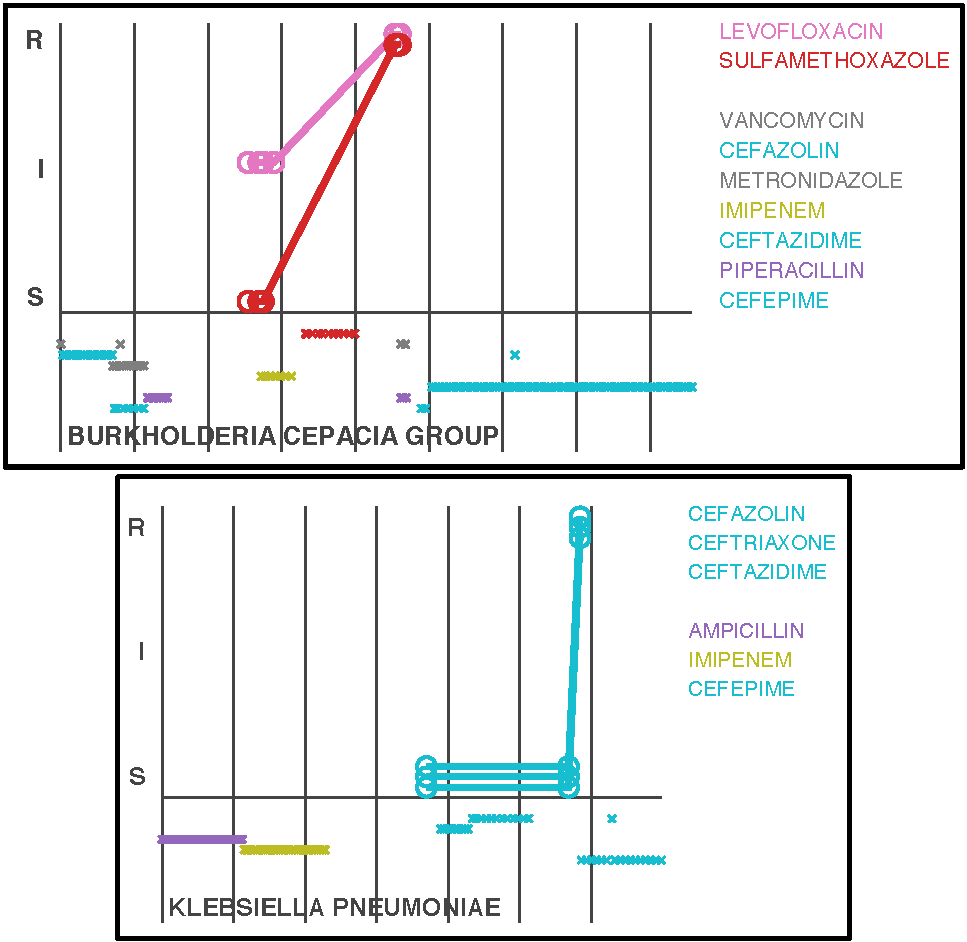
\includegraphics[width=0.8\textwidth]{chap7/dst-flip}
  \caption[Cases of emerging resistance mined from electronic medical records]{\textbf{Cases of emerging resistance mined from electronic medical records.} Records of 317,240 blood cultures performed at Mount Sinai between 2009 and 2014 were mined for same-species isolates captured during a contiguous hospital visit that showed at least one susceptible-to-resistant transition in Vitek (bioMeríeaux) drug susceptibility test (DST) results for at least one antibiotic. Two representative examples are plotted here. Time is displayed on the X axes, with each vertical line representing one week and $t=0$ representing the admission timestamp. DST results for the antibiotics involved in at least one transition are plotted as the circles above the X axis. Recorded administrations of antibiotics, colored by antibiotic class, are marked with crosses below the X axis, and vertically ordered using the order of the legend. Note that the transition time periods correspond to concurrent administrations of antibiotic(s) of the same class. S, susceptible; I, indeterminate; R, resistant.
  }
  \label{fig:dst_flip}
\end{figure}
fluoroquinolone restriction associated with decreases in fluoroquinolone-resistant \emph{C. difficile} incidence and NGS-detected transmissions\autocite{Dingle2017}, the PSP could precisely examine the impact of antimicrobial stewardship programs at Mount Sinai on the molecular evolution of local HAI strains. These future directions are currently being pursued by colleagues in the Bakel lab.

\subsection{The need for better clinical informatics}

Ultimately, as also hinted at by Chapter \ref{chap:cdi_cost}, measuring the impact of interventions at the hospital level continues to be constrained by the quality, accessibility, and depth of clinical informatics data. One could argue that the least-developed part of the vision originally introduced in Figure \ref{fig:emr_ngs_loop}, despite all of the progress evidenced in Chapters \ref{chap:steno}-\ref{chap:pathogendb}, is the development of comprehensive ``Management Strategies'' as a result of our analyses. I could certainly report transmissions along with other associations in our data, but justifying any specific response based on this information is an open question. For example, despite my best efforts to model \emph{C. difficile} risk among variables in the EMR, I quickly faced dwindling statistical power and interpretability when trying to reformat modeled risk parameters into concrete practice recommendations. This is because EMR data is observational, the hierarchy of entered data is subject to many varieties of bias, and every variable has dozens of hidden correlates. For example, even if administration of promethazine is a top ranking correlate for CDI at Mount Sinai according to our models (and it was, for four out of five CDI definitions) it would be somewhat ridiculous to suggest that banning use of promethazine, a preoperative sedative, will decrease rates of CDI.\footnote{Our best guess for why this variable ranks so highly is that it correlates with surgeries, and many surgical procedures do in fact increase the risk of CDI by incurring rounds of antibiotic prophylaxis and increased exposure to the hospital environment.}

Furthermore, I was only able to estimate a correlate for the cost of CDI: the changed length of stay, not a true dollar figure. This is certainly better than no figure at all or a regional estimate, but it is easy to imagine individual situations in which differences in the length of stay do not correlate well with true costs, either because of expensive procedures resulting from CDI (like a colectomy) or downstream effects at future visits to hospitals. The pursuit of better cost data might seem dogged and perhaps foolhardy, but as US healthcare providers incur more of the financial risk of managing populations\autocite{Shortell2015} it is impossible to expect them to rationally manage resources without attempting to understand the true costs of care at an individual level.\autocite{Hilsenrath2015} This flies in the face of most current hospital billing practices, which often purposefully obscure the true costs of care in order to set high prices that maximize payout from insurers.\autocite{Hilsenrath2015} An unfortunate side effect is that diagnosis and procedure codes created during the billing mechanism are likely skewed toward values that incur higher reimbursement.\autocite{Rhee2015,Romano1994} Unless these practices change, the ability to estimate per-patient costs will continue to suffer.

Therefore, integrating cost and clinical informatics data into models that allow infection control staff to analytically propose management strategies remains a challenging endeavor. Even operating on EMR data alone, as I did in Chapter \ref{chap:cdi_cost}, required clearance of substantial technological and bureaucratic hurdles. Although technology that supports data warehouses for EMR and clinical microbiology data has been available for some time,\autocite{Isniewski2003} in practice, making best use of these data requires a substantial amount of validation, curation, and indexing that no vendor will ever be able to provide in an ``out-of-box'' solution, as every practice environment has its unique operational quirks. In our case, I encountered irregularities in the data resulting from overaggressive deidentification procedures, shifting report formats due to an upgrade of the Vitek software, and many duplicated lab results that needed to be merged, among other issues. All of these required custom software engineering before I could begin analysis. On top of this, most infection control analyses (like those performed by the PSP) will need a partially-identified dataset, since epidemiological assessment of outbreaks requires real locations and times and these are considered identifiers for protected health information according to the HIPAA Privacy Rule.\footnote{See \href{https://www.law.cornell.edu/cfr/text/45/164.514}{45 CFR §164.514(b)(2)}.} This complicates institutional approvals for accessing large EMR datasets, and depending on the warehousing and deidentification techniques used, it may even make it impossible to associate the EMR data with specimens that are sent to the clinical microbiology lab.

Should a team like the PSP become increasingly efficient at integrating new data sources and training new statistical models on the entire dataset, the notion of a continuously learning healthcare system for infectious diseases is still within reach. It remains constrained by the dangers of inferring causality from observational data,\autocite{Dahabreh2014} since it is very unlikely that a hospital would be able to perform randomized clinical trials for all of its infection control interventions (and it would certainly be unethical to randomize exposure of patients to known HAI sources, which would seem to be necessary to definitively prove that a preventative measure works). However, to the extent that comprehensive models can be constructed from EMR data (Chapter \ref{chap:cdi_cost}) that are monitored before and after interventions are deployed, the PSP could determine to the best possible extent how much of an impact each intervention has on HAI rates and outcomes and rationally deploy these interventions in response to early-warning systems for detecting patient-to-patient transmissions in real time (Chapter \ref{chap:pathogendb}). There is no doubt that this will require substantial investment at the health system level, given the ongoing costs of building and maintaining the infrastructure for all of these data sources.

\subsection{New technologies for profiling the host response to infection}

For over a hundred years, clinical microbiology techniques have focused almost exclusively on culturing and phenotyping the pathogen and not the host.\autocite{Didelot2012} While studies of cancer and neurodegenerative diseases have pushed aggressively toward using omic techniques like RNA-seq to profile the host for diagnostic and prognostic purposes,\autocite{Costa2012} corresponding uses for infectious diseases have been slower to emerge, perhaps because the pathogens themselves have been such conducive targets. However, given our natural ability to trace infectious diseases to a root perturbation of the host—namely the introduction of a specific pathogen—it only seems logical to apply similar omic assays on hosts at proceeding timepoints to reveal biomarkers for the various outcomes of that perturbation and create the capacity to predict them. In diseases where there are a wide range of outcomes, such as viral diseases where most infections are asymptomatic but a rare few are eventually lethal, this could have direct prognostic value. For infections where the innate immune reponse is not well understood, these methods could eventually lead to a better understanding of the mechanisms underlying better and worse outcomes.

Chapter \ref{chap:chik} used three omic techniques to comprehensively profile the host response to CHIKV infection. From a research perspective, this study is valuable simply for providing the most global look at molecular and cellular perturbations induced by the virus, as it produced new signatures at the cellular and serum cytokine levels that consistently centered on monocytes, found that B cells expressed globally significant levels of CHIKV surface protein during infection despite no prior evidence for B cell tropism, and identified specific gene modules that associate with acute infection and higher viremic load. It also valiantly attempted to synthesize this maelstrom of changes into a more intepretable picture (Figure \ref{fig:multiscale_network}).

The study also attempted to tie omic changes to clinical variables like convalescent IgG titers and acute phase symptom severity, although the signatures for these changes were constrained to one assocation among CyTOF subpopulations and two small transcriptomic signatures. These signatures merit re-investigation in a large cohort to assess their reproducibility. In developing these signatures, I was constrained by the cohort design, which tried to maximize the acute-convalescent contrast while minimizing other contrasts, since the acute-convalescent signature was considered most important. In hindsight, given the overwhelming strength of the observed signature for timepoint, the study may have benefitted from a cohort that had more variation in disease severity if a substantial signature for that outcome variable were desired. Most interestingly, once follow-up data on these cases become available, if chronic symptoms develop in any of the patients (at the time of the study, they had not) it would be worthwhile to search for a new signature for this particularly worrisome outcome. Previous profiling studies followed cohorts for a year or more to identify some potential biomarkers for chronic post-CHIKV arthralgia,\autocite{Poo2014,Chaaitanya2011,Hoarau2010,Schilte2013} but given the extent of our dataset, globally significant markers could be determined with much more confidence. Follow-up samples for a far off timepoint (like one year post-infection) may also establish a baseline picture that mitigates potential criticism that the convalescent samples were not representative of a truly ``healthy'' state, although symptoms and viremia had resolved for all patients in our particular cohort.

Some of the other results would benefit from validation in more focused experiments. While the B cell expression of CHIKV surface protein is suggestive of viral entry and replication, given that B cells have not yet been found to be productively infectable by CHIKV in vitro,\autocite{Her2010,Sourisseau2007,Teng2012a} it would help to reassess some samples with antibodies for both CHIKV surface and nonstructural proteins.\footnote{Concurrent expression of nonstructural \emph{and} surface proteins is better evidence of entry and active replication, rather than surface proteins alone, which may only reflect virions bound to the outside of cells.} The subpopulation of CD14\sups{+} monocytes that associated with acute infection but displayed a previously unreported phenotype (positivity of CCR4, CXCR3 and CCR6, which are better associated with T cells) would benefit from isolation and characterization in vitro via standard flow cytometry, both to confirm that this phenotype is real and to see whether it can be directly induced from inactive CD14\sups{+} monocytes after inoculation with CHIKV. The association of several HLA transcripts with clinical variables was mechanistically plausible, but the strong association between the little-understood gene \emph{MXRA7} and symptom severity was surprising. Given that I used a very simple rubric for severity in a relatively homogenous cohort, this result should be validated by either RNA-seq or RT-PCR on samples from a larger, more heterogeneous cohort. If the result holds up, it would be interesting to assess gene expression of \emph{MXRA7} among leukocyte subpopulations during in vitro infection, so as to start narrowing down what its role in the innate immune response might be.

All of these experiments are plausible lines of future inquiry by the Dengue Human Immune Profiling Consortium, which also plans to develop comprehensive immune profiles for other arboviral infections. Once this profiling is complete for all \textasciitilde 200 biosamples (in approximately three years), a unified network model for all three diseases will be attempted, and the sample size will also then be sufficient for fitting Bayesian models on coexpression modules that strongly associate with the various clinical outcomes. Bayesian models permit the inference of causality between differentially expressed genes and the identification of key drivers for the innate immune response. In short, I believe that the potential applications of this dataset and the involved immune profiling techniques have only just begun to be explored.

\section{Conclusions}

\newthought{The introductory chapter} of this dissertation claimed, ambitiously and with only extrapolations as evidence, that ``a potent combination of NGS and EMR data will transform infectious disease management.'' Although this thesis has not singlehandedly completed that transformation, I find no reason to change this prediction, given the substantial progress that was demonstrated here for a few short years of effort. As I had expected, the unprecedented specificity of the PSP's NGS data allows us to reconstruct and detect clandestine transmissions of HAIs within The Mount Sinai Hospital, and large parts of this process are now automated and easily communicated to clinicians with the software that we have built. The use of long read NGS and \emph{de novo} assembly to support pathogen surveillance is novel—and moreover, looks to be essential for characterizing the recombination and horizontally transferred genes that underlie evolution of virulence and antibiotic resistance in HAI organisms, particularly given the diversity of many gram negatives. As the PSP's linked dataset of genomes and clinical metadata grows, I still fully expect that the PSP can develop predictive models for virulence, resistance, and infection outcomes based on comprehensive, pan-genomic analyses. Given continued investment in the clinical informatics available to the PSP, it will be able to establish the local costs of other HAIs, measure effects correlated with various interventions, and support specific recommendations for new management strategies. Meanwhile, technologies available for profiling the host response to infection continue to grow, and my study of chikungunya virus indicates that omic assays can simultaneously establish globally significant trends in the immune response (like the dominance of monocyte involvement) and extremely subtle biomarkers for clinical outcomes, like infection severity.

In conclusion, this dissertation found that integrative analysis of EMR, NGS, and other omics data was an fruitful strategy for addressing critical components of several urgent problems in infectious diseases, such as the spread of HAIs, increasing rates of antimicrobial resistance, and comprehensive profiling of the host response to a newly epidemic, poorly understood virus. Therefore, I believe that multiscale analysis is indeed transforming clinical infectious diseases.